\documentclass[pdftex,12pt,a4paper]{report}

\usepackage[pdftex]{graphicx}
\usepackage{float}
\usepackage{fancyvrb}
\fvset{xleftmargin=2em}

\usepackage{pgfplots}
\pgfplotsset{width=10cm,compat=1.9}
\usepackage{tikzscale}
\usepackage{pgfplotstable}
\usepackage{booktabs}
\usepackage[font=small,labelfont=bf,tableposition=top]{caption}

\usepackage[utf8]{inputenc} % isto é um comentário
\usepackage[portuges]{babel}
\usepackage[T1]{fontenc}
\usepackage{times}
%\usepackage{lmodern}
\usepackage[obeyspaces,spaces]{url}
\usepackage[left=25mm,right=25mm,top=25mm,bottom=25mm]{geometry}
\usepackage{titlesec}
\usepackage{mathtools}
%identa 1º paragrafo de capitulos e secções
\usepackage{indentfirst}

\newcommand{\HRule}{\rule{\linewidth}{0.5mm}}
\titleformat{\chapter}{\normalfont\huge}{\thechapter.}{20pt}{\huge}


\begin{document}

\begin{titlepage}


\begin{minipage}{0.3\textwidth}
\begin{flushleft} 

\includegraphics[width=\textwidth]{logo.png}
\end{flushleft}
\end{minipage}
\begin{minipage}{0.6\textwidth}
\begin{flushright} 

\textsc{Departamento de Engenharia Informática}\\[0.1cm]
\bfseries Mestrado Integrado em Engenharia Informática \\ [0.1cm]
\bfseries \textit{Computação Gráfica}\\[8mm]

\end{flushright}
\end{minipage}


\vspace{3cm}


\begin{center}


\LARGE Fase 2

\Large \textbf{\textit{Geometric Transforms}}\\[1.5cm]


{\Large \bfseries Grupo 18\\[2cm] }


\noindent\begin{minipage}[b]{.3\textwidth}
	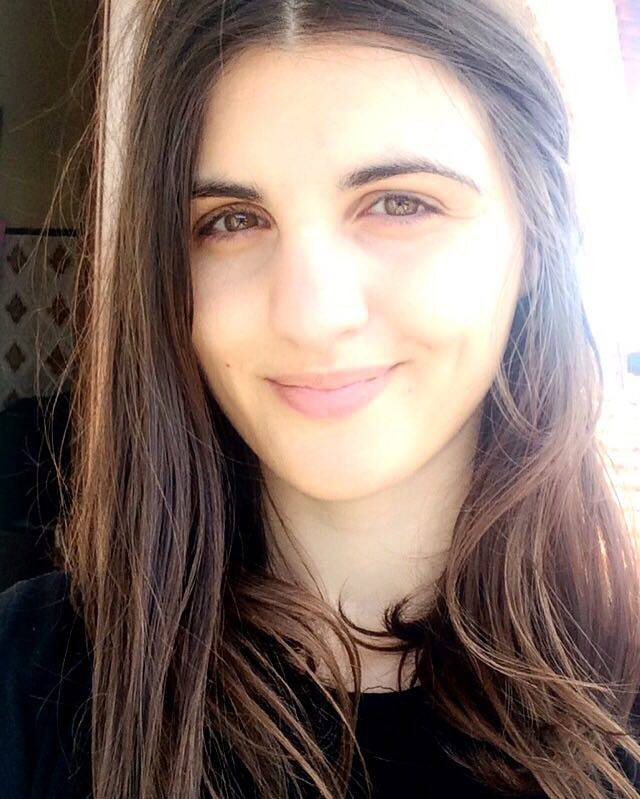
\includegraphics[scale=0.2]{celia}
	\small{Célia Figueiredo a67637}
\end{minipage} 
\hfill
\begin{minipage}[b]{.3\textwidth}
	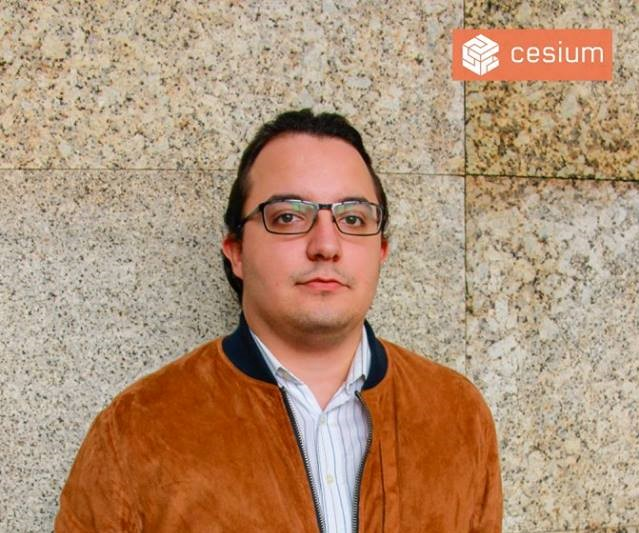
\includegraphics[scale=0.3]{luis}
	\small{Luís Pedro Fonseca a60993}
\end{minipage}




\vspace{3ex}


\vfill

\large Braga, {\large \today}

\end{center}
\end{titlepage}


\tableofcontents

\begin{abstract}

O presente relatório descreve o trabalho efetuado para a realização da quarta fase do projeto, onde foi pedido a implementação e representação de um Sistema Solar com o uso da ferramenta \textit{OpenGL}. Nesta fase é preciso implementar texturas nas diversas esferas para as conseguirmos destinguir umas das outras. É preciso
criar também a iluminaçãoo dos diversos planetas e é para este ponto que
vamos precisar de calcular as normais das diversas formas geométricas.
\end{abstract}
\chapter{Introdução}
\label{cap:intro}

No âmbito da Unidade Curricular de Computação Gráfica pertencente ao plano de estudos do 3º ano do Mestrado Integrado em Engenharia Informática foi proposto o desenvolvimento de um sistema solar. 

Concluída a primeira fase tem-se agora de introduzir transformações geométricas, \textit{translate}, \textit{rotate} e \textit{scale}, ao projeto. Assim, nesta fase, o \textit{engine} deverá ser capaz de realizar translações, rotações e escalas das várias figuras a desenhar.
As transformações geométricas a realizar deverão ser especificadas no ficheiro XML, seguindo um formato definido, assim como as figuras a desenhar.

A demonstração para a segunda fase é um modelo estático do sistema solar com o Sol, Planetas e Luas definidos em hierarquia.

\chapter{Iluminação}

Com o objetivo de obter mais dinamismo do cenário, implementou-se iluminação. Para tal, e como todas as figuras estão a ser geradas ponto a ponto, sem recurso aos modelos já oferecidos pelo \textit{OpenGL}, foi preciso especificar as normais de cada objeto. Além disso, foi necessário expandir as funcionalidades do \textit{xml} para obter informação relativamente aos materiais dos objetos, ou seja a forma como reagem com a luz, bem como as luzes em si.

É com os vetores das normais que nós definimos como  a luz é refletida por determinado objeto, isto é, com a emissão da luz de determinado ponto é necessário saber se quando esta luz atinge o objeto como é que o ilumina.
Quando falamos de iluminação o existem vários tipos de iluminação que podemos usar para iluminar um objeto:

\begin{itemize}
	\item Difusa;
	\item Ambiente;
	\item Especular;
	\item Emissiva;
\end{itemize}


\section{Luzes }

No nosso caso, fizemos a implementação que permite a um dado objeto ser incidido com um dos tipos de luz, para tal, temos no \textit{xml} a \textit{tag} luz.
Na \textit{tag} luzes definimos os tipos de luzes que são aplicadas ao planetas quando este recebem a luz que é emitida pelo sol, pois no sistema solar o sol não é ”iluminado”, mas sim uma fonte de luz. Para definirmos a luz no sol usamos pontos que se encontram ”dentro” da área representada pelo sol no \textit{xml}.
portanto um conjunto de luzes. que são desenhadas antes dos objetos do mesmo grupo. Utilizar-se-á uma luz para evitar aumentar a complexididade do sistema, como tal só se faz \textit{enable} a \textit{lightning} e \textit{light0}.


\section{Materiais}

De forma a ajustar como os objetos reagem à luz, foi necessário introduzir materiais. 

Os materiais são diferentes, pois nos materiais temos que cada modelo possui o seu próprio material. Para isso definimos uma  estrutura de dados que nos permite aramazenar as características que cada modelo tem para o material, isto é, para cada material temos de armazenar o modelo em causa, qual o material associado a esse modelo, qual a cor desse
modelo. 


\section{Normais}

As normais servirão para se ativar a funcionalidade de iluminação de cada figura geométrica. É graças a estas que é possével determinar o ângulo de incidência da luz e como tal variar a intensidade observada.
Foi necessário adicionar o glEnable(GL\_NORMALIZE) para recalcular as normais após um \textit{glScale}.


\subsection{Esfera}

Para a Esfera, as normais são os próprios pontos. Como as normais são um vetor não se torna necessário retirar o raio dos pontos. Desta forma, como as coordenadas do ponto são relativas ao seu centro, é exatamente esse vetor que define a sua normal.

\begin{verbatim}
int drawSphere_VBO(float radius, float centerX, float centerY, 
float centerZ, int stacks, int slices, Ponto3D points, int* indexes, 
Ponto3D normals){

// calculo do angulo de cada slice e stack, pasado para radianos
divBeta = (360.0f / (float) slices) * M_PI / 180.0f;
divAlpha = M_PI / (float) stacks; 	// == (180.0f / (float) stacks) * M_PI / 180.0f;

// criação dos arrays com os angulos todos os slices e stacks sendo que os iniciais sao predefinidos
// os angulos alpha (do Norte ao sul) começam em 90 e vao até -90, i.e., PI/2 e vão até -PI/2
alphas[0] = M_PI / 2.0f;
alphas[stacks] = - M_PI / 2.0f;
// os angulos beta (horizontal) começam no 0 até 360, i.e., de 0 a 2PI
betas[0] = 0;
betas[slices] = 0;

for(i = 1;i < slices;i++)
betas[i] = betas[i-1] + divBeta;
for(i = 1;i < stacks;i++)
alphas[i] = alphas[i-1] - divAlpha;

// Triangulos do topo da esfera
stHeightDown = radius * sin(alphas[1]);
stHeightUp = radius * sin(alphas[stacks - 1]);	
radDown = radius * cos(alphas[1]);
radUp = radius * cos(alphas[stacks - 1]);	
     Calcula o ponto do topo da esfera; 
     Calcula a normal nesse ponto; 
     Calcula o segundo ponto  esfera; 
     Calcula a normal nesse ponto; 
     Guarda pontos e normais; 
indp += 2;
for(i = 1;i < slices; i++) {
    Calcula o ponto seguinte da stack da esfera;
    Guarda o ponto; 
    Calcula a normal para esse ponto; 
     Guarda a normal calculada 
      Incrementa o indice; 
       Desenha triâgulo; 
      Incrementa o indice dos indices; 
}
   desenha o último triangulo da stack; 
   Incrementa o indice dos indices; 

// resto da esfera
 for(i = 2;i < stacks;i++){
     Calcula o ponto seguinte da stack da esfera;
     Guarda o ponto; 
 for(j = 1;j < slices;j++) {
      Calcula as normais dos quadrados a desenhar 
       desenha quadrado ; 
       indi += 6;
  }
     desenha quadrado ; 
    indi += 6;
}

// Triangulos da base da esfera
stHeightUp = radius * sin(alphas[stacks - 1]);
radUp = radius * cos(alphas[stacks - 1]);
  Calcula o ponto do topo da esfera; 
   Calcula a normal nesse ponto; 
indp++;
for(i = 1;i < slices; i++) {
  desenha triangulo; 
  indi += 3;
}
  desenha triangulo ; 
  indi += 3;
return indp;
}
\end{verbatim}


\subsection{Plano}
As normais do plano criado na horizontal, ou seja em que o y não varia, são fáceis de se calcular. As normais dos quatro vértices do apontam para 0 1 0.

\subsection{Box}
Para as normais dos oito vértices da box temos de ter em mente que cada vértice vai ter três normais diferentes, referente às três faces da box que estes fazem parte. Por isso especificou-se as normais por face. Cada face tem portanto as normais à semelhança do plano, com só uma das coordenadas a 1 e as outras a 0.

\subsection{Cone}
É preciso ter-se em atenção os ângulos dos diversos pontos do Cone.
Conseguindo-se desenhar o Cone a diferençaa do x e z dos diversos pontos e as suas respectivas normais é  que só precisamos dos senos e cosenos, não os multiplicamos pelo raio. Os y de todas as normais calculam-se da mesma maneira: divisão entre a altura do cone e a raiz quadrada entre a soma do quadrado da altura com o quadrado do raio.


\subsection{Torus}

Antes de calcular as normais do tórus, é necessário perceber o que deve ser esperado. Como não se estão a implementar sombras (uma objeto à frente da luz, escurecer o que está a trás de si, um tórus quando horizontal perante a luz, deve ter 2 superficies iluminadas. Ou seja, ao contrário de uma esfera que os seus vetores são relativos ao ponto central, um tórus deve ser analisado como um cilindro em que os vetores são relativos ao eixo à volta. Desta forma, consegue-se obter simultaneamente a parte exterior e interior
iluminada de acordo com a posição da luz.




\section{Texturas}

As texturas são armazenadas de modo a que quando o ficheiro é lido saber o tipo de textura que o objeto vai ter.


Nas texturas  temos duas vertentes, isto é, temos a aplicação de uma imagem como textura, mas temos também uma vertente, que é a definição do sistema solar que não é definir as texturas como imagens, mas sim ter uma espécie de material, isto é ter o sistema solar em que cada planeta possui um material definido por nós.
O carregar de uma textura é feito através da leitura no \textit{xml}de um campo textura que indica o nome da textura a carregar.





\chapter{Motor}
\label{cap:p2}

O \textit{engine} tem como principal função apresentar o modelo gráfico. Para
tal utiliza-se a biblioteca \textit{GLUT (OpenGL Utility Toolkit )}, em conjunto com
a biblioteca gráfica \textit{OpenGL}.


\section{Objectivos}

Com o motor pretende-se uma aplicação que seja capaz de ler um conjunto de pontos especificados em ficheiros XML e .3d e os desenhe numa janela. Além desse objetivo principal foi incluída uma câmara em torno do objeto desenhado e um menu simples que permite alterar o modo de visualização dos pontos.

Nesta secção apresenta-se de que forma o motor foi desenvolvido, começando-se por explicar a leitura dos ficheiros

\section{Leitura Ficheiros}

\subsection{Ficheiro XML}

A estrutura do ficheiro XML contempla apenas dois tipos de elementos:

\begin{itemize}
	\item[\textbf{scene}] - elemento pai
	\item[\textbf{model}] - elemento com 1 atributo \textit{file} cujo valor corresponde ao nome de um ficheiro de pontos
\end{itemize}



O pseudo-codigo da função de leitura do XML pode ser expresso da seguinte forma:

\begin{Verbatim}
vector<const char *> leXML() {
	Abre documento para leitura
	
	if (nao houve erro a abrir o ficheiro) {
		Acede ao primeiro elemento filho de "scene" 
		(que é um elemento "model")
		
		while (houver elementos "model") {
			Vê qual o valor do primeiro atributo 
			do elemento
			
			Coloca o valor do primeiro atributo do
			 elemento no resultado
			 
			Avança para o proximo elemento
		}
	}
	else {
		Informa erro a abrir o ficheiro
	}
	
	Retorna resultado
}
\end{Verbatim}

\subsection{Ficheiros .3d}


Ns ficheiros .3d, cada linha representa um ponto. Em cada linha, existem 3 valores, separados por espaço, correspondentes às coordenadas cartesianas do ponto. É necessário por isso ter uma função que seja capaz de ler os pontos destes ficheiros para que o motor os possa desenhar.

No main está um pedaço de código que permite a leitura destes ficheiros, que recebe como parâmetro o nome de um ficheiro e coloca os pontos do ficheiro num vector de pontos (que é uma variável global). Este vector de pontos será depois o que o motor vai utilizar para desenhar os pontos.

A parte do código que lê o ficheiro XML funciona da seguinte forma:

\begin{Verbatim}

if(xml = fopen(argv[1],"r")) {
lê a primeira linha, verifica abertura do scene
while(consegue ler do xml) {
procura os model files e guarda os nomes 
}
	fclose(xml);

 } else {
 perror(Impossivel abrir XML);}
 
 
\end{Verbatim}

\section{Desenho dos pontos}

O resultado da leitura do XML e dos ficheiros .3d nele especificados é um conjunto de \textit{Ponto3D} que são armazenados numa variável global. Este conjunto de pontos está implementado sobre a forma de um \textit{array<sPonto3D>} que é uma variável global ao programa.

A ordem pela qual os pontos aparecem no vector é a ordem pela qual apareceram nos ficheiros, que por sua vez é a ordem pela qual deverão ser desenhados. Nesta situação, desenhar os pontos corresponde simplesmente a percorrer todos os pontos colocados no vector e a pedir ao GLUT para os desenhar. Mostra-se um excerto de código da função \textit{renderScene()} que corresponde ao desenho dos pontos:

\begin{Verbatim}

glBegin(GL_TRIANGLES);
glColor3f(0.0, 0.0, 1.0);

for(i = 0;i < _buffer_size;i++){
glVertex3f(_buffer_pontos[i].x,_buffer_pontos[i].y,
_buffer_pontos[i].z);
}

glEnd();
\end{Verbatim}

Assume-se que os ficheiros .3d já contêm a ordem correta dos pontos a ser desenhados.

\section{Câmara}

Para se poder ver o objeto desenhado de vários ângulos foi implementada uma câmara.  Visto que a posição da câmara é ------ para gerir o movimento da câmara.


À função \textit{gluLookAt()} são passadas -----

\begin{Verbatim}
gluLookAt(xcam, ycam, zcam,
xcam+lx, ycam+ly,  zcam+lz,
0.0f, 1.0f,  0.0f);
\end{Verbatim}

É possível ao utilizador mudar a posição da câmara. Os controlos são os seguintes:

\begin{itemize}
	\item[\textbf{Tecla 'W'}] permite ao utilizador ir para cima
	\item[\textbf{Tecla 'S'}] permite ao utilizador ir para baixo
	\item[\textbf{Tecla 'A'}] permite ao utilizador ir para a esquerda
	\item[\textbf{Tecla 'D'}] permite ao utilizador ir para a direita
	\item[\textbf{Tecla 'Q'}] permite ao utilizador afastar-se  para cima do objeto
	\item[\textbf{Tecla 'E'}] permite ao utilizador aproximar-se para baixo do objeto
\end{itemize}

Estas operações traduzem-se em operações sobre a câmara disponibilizadas pela classe \textit{CoordsEsfericas}:

\begin{Verbatim}
void processNormalKeys(unsigned char key, int xx, int yy) {

float fraction = 0.1f;

switch (key) {
case 'd' :
angleX += 0.01f;
lx = sin(angleX);
lz = -cos(angleX);
break;

case 'a' :
angleX -= 0.01f;
lx = sin(angleX);
lz = -cos(angleX);
break;

case 'w' :
angleY += 0.01f;
ly = sin(angleY);
break;

case 's' :
angleY -= 0.01f;
ly = sin(angleY);
break;

case 'q' :
ycam = (ycam + 0.5);
break;

case 'e' :
ycam = (ycam - 0.5);
break;
}
glutPostRedisplay();
}


\end{Verbatim}

Quando a função \textit{gluLookAt()} é chamada e acede aos valores de x, y e z da posição da câmara, estes estão atualizados.

\section{Menu}

Para proporcionar alguma flexibilidade na visualização das figuras desenhadas foi incluído um menu que permite ao utilizador alternar entre o modo de visualização de pontos, linhas, ou objeto preenchido:


O menu foi construído da seguinte forma:

\begin{Verbatim}
glutAddMenuEntry("FILL", 0);
glutAddMenuEntry("LINE", 1);
glutAddMenuEntry("POINT", 2);

case 'f' :
_polygon_mode = GL_FILL;
break;
case 'g' :
_polygon_mode = GL_LINE;
break;
case 'h' :
_polygon_mode = GL_POINT;
break;
\end{Verbatim}










\chapter{Conclusão}

Nesta fase procedeu-se a vários ajustes a nível da estrutura das classes,
mas também otimizaçõess de código. Assumir isto como uma prioridade significou aliviar a implementaçãoo de novas funcionalidades futuras que podem
ser mais exigentes a nível de processamento. Culmatou-se desta forma alguns
dos problemas de desorganizaçãoo do código apresentados anteriormente.

Assim sendo introduziu-se VBOs no modo que os pontos são guardados,
e separou-se este processo para uma classe distinta do engine. Resolveu-se
também o problema de recarregamento dos ficheiros sempre que se fazia
render.
Foram realizadas algumas alterações a nivel da câmara, dando um maior
controle ao utilizador, permitindo, para além do que já podia realizar na
primeira fase, fazer zoom in e zoom out e melhorou-se a rotação da câmara. 

Continua a não ser possivel diferenciar por cores as diferentes figuras,
sendo estes um dos aspectos que queremos melhorar nas seguintes fases.
Existem, também, ainda alguns problemas de otimização, tal como a leitura
repetida de ficheiros iguais. Por exemplo, para dois planetas definidos
pelo mesmo ficheiro, a estrutura carregada terá essa informaçã repetida, e
o ficheiro será lido duas vezes.
Em suma, achamos que, com esta fase 2, definiu-se as estruturas base
a utilizar e simplificou-se a introdução de novas funcionalidades tendo-se
melhorado as funcionalidades já existentes.


\end {document}


